\documentclass{article}
\usepackage[utf8]{inputenc}
\usepackage[]{amsmath}
\usepackage{amsthm,amssymb}
\usepackage{enumerate}% http://ctan.org/pkg/enumerate
\usepackage{hyperref}
\usepackage{tikz}
\usepackage{ mathrsfs}
\usepackage[margin=0.5in]{geometry}
\usepackage{graphicx}
\usepackage{tikz}
\usepackage{pgfplots}

% no indents pls
\setlength\parindent{0pt}


%%% defs for theorem environments
\renewcommand{\qedsymbol}{\rule{0.7em}{0.7em}} % black box for QED
\newtheorem*{thm}{Theorem}
\newtheorem{lem}{Lemma}
%defining style for Cases
\newtheoremstyle{casestyle}{\topsep}{1pt}{}{0pt}{\itshape}{.}{5pt plus 1pt minus 1pt}{}
\theoremstyle{casestyle}
\newtheorem{case}{Case}
%smallcaps-ing "Proof" header
\let\oldproofname=\proofname
\renewcommand{\proofname}{\rm\sc{\oldproofname}}

\begin{document}

\section *{Problem 4}
\begin{enumerate}[i]
\item Encoding skiplist as multiway tree. Let each node in a skiplist be of level $1$ to $k$, where level $i$ indicates that the node has $i$ forward pointers, from $1$ to $i$. We begin with a skiplist $L$ with $n$ nodes and a highest level of $k_{\max}$ (this is the level of the node in $L$ with the highest level). To encode $L$ as a multiway tree $T$, we start at level $k_{\max}$; all of the nodes with a level of $k_{\max}$ are keys in the root node of $T$. We then continue down the levels in the same way: each node of level $k$ in $L$ will translate to a key in a node of depth $k_{\max}-k$ in $T$. The nodes on this level $k$ that are not separated by any nodes of level $>k$ are clustered together in the same node $j$ in $T$ as keys. The parent of $j$ is the node of depth $k_{\max}-k-1$ in $T$ such that the range of keys in $j$ falls into the ``key space'' of that node, as explained in lecture 5. The root node has no parent. We repeat this until level $1$, the bottom of $L$ and the encoding is complete. If no appropriate parent in the level immediately above can be found, keep traversing up levels until a parent can be found. This can be shown in the diagram, in which the node with ``4'' starts out as level 1 nodes, but is a direct child of the root node, since there is no other node of level 2 between the ``3'' node and ``5'' node \\\\
Encoding a multiway tree as a skip list. Let $k_{\max}-1$ be the maximum depth of the tree $T$ that will be encoded to list $L$. We begin by creating a simple linked list of all the items in sorted 
order. We then start from depth $k_{\max}-2$ in $T$ and link together (with forward pointers)/elevate (to level $2$) nodes in $L$ that correspond to keys in nodes of depth $k_{\max}-2$  in $T$. We repeat this process, linking together nodes in $L$ and elevating them to level $i$ for every depth $k_{\max}-i$ in $T$ until depth $0$. Note that ``elevation'' occurs as a side effect of the linkage and is not an independent process in itself.
\\\\
Note that while this creates an isometry between the skiplist and multiway tree, it is possible that converting a skiplist to multiway tree and back does not result in the original skiplist. This is due to the fact there may be levels of the skiplist with the exact same nodes and thus no meaningful corresponding node in the tree i.e.\ there are more skiplists than valid multiway trees. This can be illustrated in the following diagram, where a skiplist is encoded to a multiway tree, which is then encoded back to the skiplist.

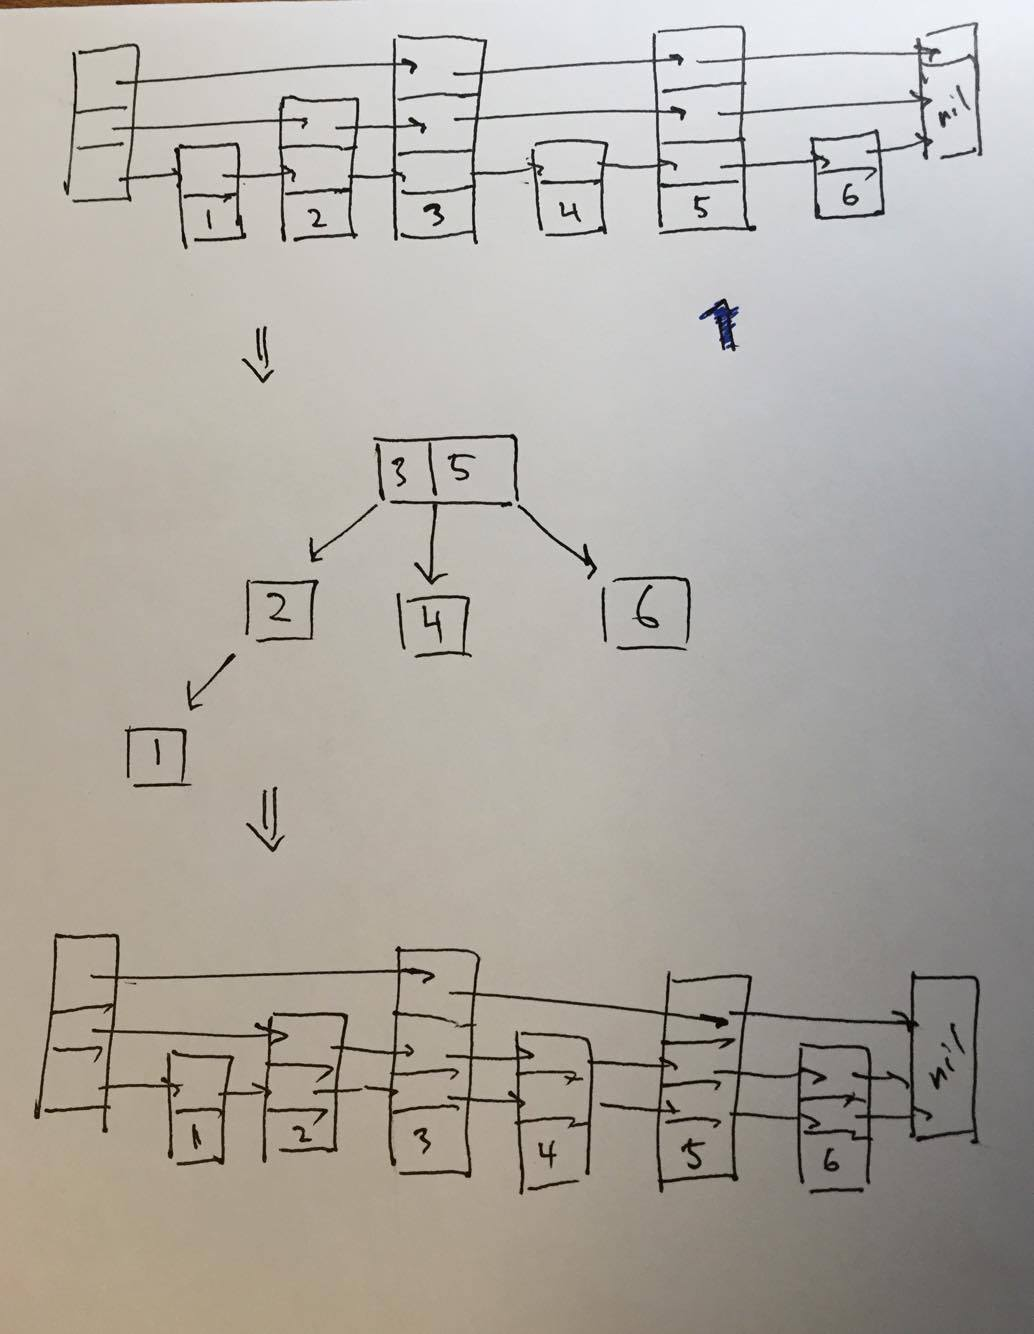
\includegraphics[scale=.3]{4i}

\item We will walk through the B-tree rules and translate as follows: \begin{enumerate}
  \item The root node has between $1$ and $2b-1$ keys $\rightarrow$ $L$ can only have $1$, $2$, or $3$ nodes linked together at the highest level $k_{\max}$.
  \item All non-root nodes have between $b-1$ and $2b-1$ keys $\rightarrow$ At every subsequent level $k_i$, there can be $1$, $2$, or $3$ nodes linked together of level $i$ between nodes of any level greater than $i$ or the two ends of the list.
  \item All leaf nodes are stored at the same depth and all root-null paths through the tree pass through the same number of nodes $\rightarrow$ At every level $i$ such that $i > 1$, there must be at least one node of level $i-1$ between every node of a level $i$ or higher or the two ends of the list.
  \item The B-tree is a BST and has sorted nodes $\rightarrow$ The nodes on level $i$ between nodes of level $i$ or higher or the two ends of the list must be sorted, have values less than the next node of level $i+1$ (unless the next node is an end node or we are at the top of the tree) and have values greater than the previous node of level $i+1$ (same conditions apply as before).
  \end{enumerate}

\item Due to the isometry between the 1-2-3 List $L$ and 2-3-4 Tree $T$, we can perform a similar algorithm to a B-tree lookup. We first traverse the nodes on the top level in $L$ sequentially until we find the key or get to a node on that level just before the key (we would have to do a lookahead to ensure this). If the key is not found, descend one level on the node where the search stopped and recursively explore that lower level in the same way, descending as needed, until the node containing the key is found. At the lowest level, no descending can be done, so we must traverse until we reach the key or overshoot and conclude that the key does not exist. This emulates a B-Tree lookup, since descending one level and following that pointer is equivalent to following a child connection in the B-Tree lookup. Thus, due to their isometry, the lookup time on a 1-2-3 List will be asymptotically identical to that of a 2-3-4 Tree lookup: $O(\log n)$ per lecture.

\item Algorithm: In order to insert element $e$. We first perform a lookup to find the location of the node, $p$ right before the element to be inserted. This is done via the same lookup mechanism as described in the previous part, with the minor modification that when we overshoot on the lowest level, we keep track of the node right before. During this traversal, we also keep track of the nodes at which a descent to a lower level occurred. \\\\ Since $p$ is guaranteed to have level 1 based on 1-2-3 List properties (property (c)), we can insert element $e$ as a node right after $p$ on the same level (level 1). We then go back and ensure that this does not violate property (b) that there can be no more than $3$ nodes of level $1$ between nodes of any level $>1$. We can check this since we kept track of the nodes at which a descent occurred. Thus, we can start from node containing the descent to level $1$, $d$ and count the number of nodes of level $1$ between $d$ and the next node with a level $>1$. If this number is $1$, $2$ or $3$, then nothing needs to be done. Otherwise, there are $4$ nodes and we elevate the third node from the left by inserting it on the level above (level 2 in this case) between $d$ and the node that $d$ points to on that level. We now perform this check on the next level to ensure that there are not $4$ nodes on level 2 and continue in the same fashion (checking against the previous descent node and elevating up) until we reach the top level $k_{\max}$. If there end up being $4$ nodes connected on level $k_{\max}$, then we elevate the third node as before (with the node connecting only to the beginning and end, ``nil'' nodes of the list on that level) and the new top level of the list becomes $k_{\max}+1$.
\\\\ Correctness: Since insertion is always after the position that the element would have been at on the bottom level, the property listed in (d) of 1-2-3 Lists is not violated by the initial insertion. In the case of an elevation of a node to a higher level, property (d) is still not violated since it is inserted into the the list of higher level in sorted order. Since elevating the third node in clusters of $4$ nodes of the same level produces two and one nodes separated by the new node, we do not violate property (a) or (b). Since we are only inserting elements and the elevation still preserves at least one node of the original level in between nodes of the new level, we do not violate property (c). Thus, after insertion, our list is still a 1-2-3 list.
\\\\ Runtime: The initial lookup takes $O(\log n)$ time as shown in the previous part. Each elevation takes constant time since each list has a maximum size of $3$ before insertion and linked list insertion is $O(1)$. In the worst case, we need to elevate every set of nodes all the way to the root - since the height of the tree is $O(\log n)$, the time taken to elevate is also $O(\log n)$. Thus, insertion takes a time of $O(\log n)$.

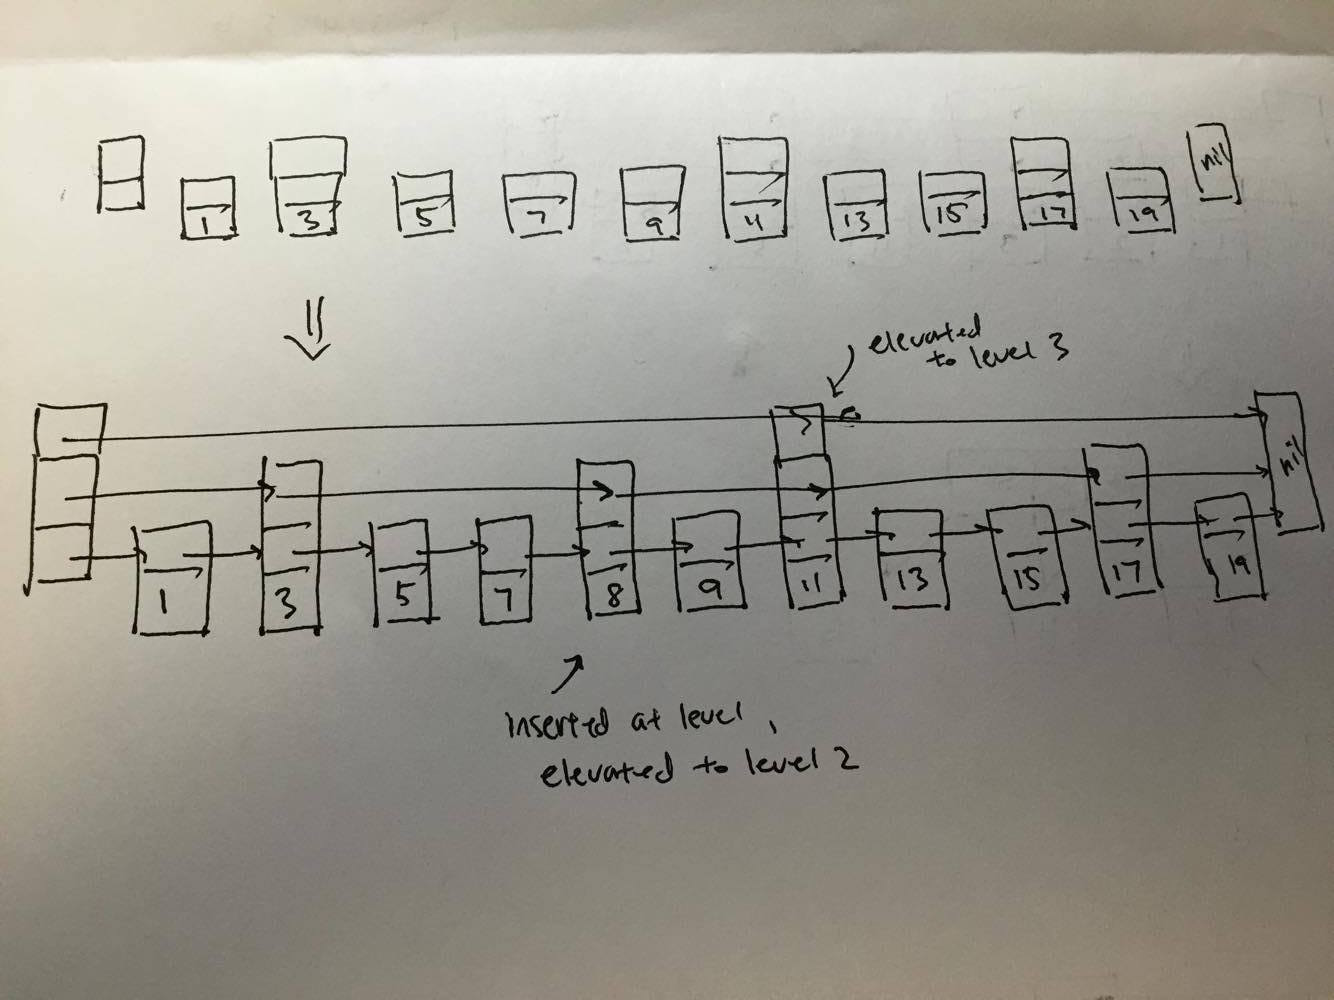
\includegraphics[scale=.3]{4iv}

\end{enumerate}

\end{document}



%%% Local Variables:
%%% mode: latex
%%% TeX-master: t
%%% End:
